\documentclass[11pt]{article}
\title{Application of network reliability using exhaustive enumeration - Project 2}
\author{Harshavardhan Nalajala}
\date{July 10 2017}
\usepackage{listings}
\usepackage{graphicx}
\usepackage{algorithm}
\usepackage[noend]{algpseudocode}
\begin{document}
\maketitle
 \tableofcontents
 \section{Description}
 
 \section{Algorithm}
\begin{algorithm}
\label{euclid}
\begin{algorithmic}[1]
\Procedure{calculateReliability}{}
\For {\texttt{i in numEdges}} 
\State $list \gets getCombinations(edges, i)$
\State for each $combination$ in $list$
\State $edgeMatrix \gets constructEdgeMatrix(combination)$
\If {$connectedUsingBFS(edgeMatrix)$} 
\State $reliability \gets reliability + probability(combination)$
\EndIf
\EndFor
\Return reliability
\EndProcedure
\end{algorithmic}
\begin{algorithmic}[1]
\Procedure{constructEdgeMatrix(combination)}{}
\For {\texttt{i in numNodes}}
\If {$\texttt{combination[i] == 0}$}
\State $s \gets \texttt{edge[i][0]}$
\State $d \gets \texttt{edge[i][1]}$
\State $\texttt{edgeMatrix[s][d] = 1}$
\State $\texttt{edgeMatrix[d][s] = 1}$
\EndIf
\EndFor
\Return $edgeMatrix$
\EndProcedure
\end{algorithmic}
\begin{algorithmic}[1]
\Procedure{getCombinations($startindex, endindex, i$)}{}
\If {$startindex = endindex$}
\If {$k = 0$}
\Return "0"
\EndIf
\Return "1"
\EndIf
\State $list = getCombinations(startindex+1, endindex, i)$
\For {\texttt{list in list}}
\State $nlist \gets "0" + list$
\EndFor
\State $list = getCombinations(startindex+1, endindex, i-1)$
\For {\texttt{list in list}}
\State $nlist \gets "1" + list$
\EndFor
\Return $nlist$
\EndProcedure
\end{algorithmic}
\begin{algorithmic}[1]
\Procedure{connectedUsingBFS(edgeMatrix)}{}
\For {\texttt{i in  numNodes}}
\State $vertex\texttt{[i]} \gets 0$
\EndFor
\State \texttt{add 0 to queue}
\While {\texttt{queue is not empty}}
\For {\texttt{j in numNodes}}
\If {\texttt{edgeMatrix[i][j] != 0 and vertex[i] != 1}}
\State \texttt{insert j to queue}
\State \texttt{vertex[j]} $\gets 1$
\EndIf
\EndFor
\EndWhile
\For {$\texttt{j in vertex}$}
\If \texttt{vertex[j] == 0}
\Return 0
\EndIf
\EndFor
\Return 1
\EndProcedure
\end{algorithmic}
\end{algorithm} 
 \section{Input}
 \begin{lstlisting}
input.txt:
5
10
1
1 2
1 3
1 4
1 5
2 3
2 4
2 5
3 4
3 5
4 5
0.05
\end{lstlisting}

\section{Output}
\begin{lstlisting}
Probability 	 Reliability
0.050000 	 0.000569
0.100000 	 0.005009
0.150000 	 0.018029
0.200000 	 0.044373
0.250000 	 0.087816
0.300000 	 0.150322
0.350000 	 0.231491
0.400000 	 0.328416
0.450000 	 0.435968
0.500000 	 0.547485
0.550000 	 0.655738
0.600000 	 0.753997
0.650000 	 0.837022
0.700000 	 0.901767
0.750000 	 0.947684
0.800000 	 0.976563
0.850000 	 0.991951
0.900000 	 0.998283
0.950000 	 0.999884
1.000000 	 1.000000
// 1024 combinations and total reliability of network with p = 0.9
Total combinations: 1024 Reliability: 0.998283
// Run k from 0 to 20, reliability values
0.998283
0.997346
0.996311
0.995507
0.995024
0.992530
0.991743
0.991043
0.990579
0.990784
0.989484
0.987036
0.987080
0.985806
0.983896
0.984593
0.982788
0.980476
0.980215
0.982170
0.979959
\end{lstlisting}

\section{Analysis}
As reliability of each link increases, overall reliability of the whole system increases since probability of each link in up state is directly proportional to overall system up state. This is depicted in graph of figure 1 at the end. \par
728 combinations belong to system up state and 295 combinations belong to system down state. Choosing a combination randomly is biased towards system up state and reversing the state will reduce the reliability. So, with increasing k, reliability of the whole system reduces gradually except one case where reliability of the system dips down with k = 19. Gradual reduction in reliability is explained based on system up random combinations chosen are greater than system down combinations. Sudden dip happened since random combinations are all system up combinations.


\section{ReadMe}
Run Makefile using following command in the directory.
\begin{lstlisting}
make -f Makefile
\end{lstlisting}
Makefile generates the executabla(reliability).
Executable expects input in the following format.
Run command: ./reliability < input.txt
\begin{itemize}
\item number of nodes, n
\item number of edges, N
\item N lines of two space separated integers i, j denoting the edge between i and j
\item initial probability, p
\end{itemize}
\section{Appendix}
Files:
\begin{itemize}
\item graph utils.h, graph utils.c: API to get the edge matrix from given combination and API implementation of BFS to check network connectivity.
\item combinations.h combinations.c: API to create all combinations of 0s and 1s, API to print and free the list of combinations. Linked list used for dynamic memory management.
\item reliability.c: Main file containing API to calculate reliability of each edge, reliability of overall system using combinations API and graph utils API.
\end{itemize}
\begin{lstlisting}
combination.h:
#ifndef __COMBINATIONS_H
#define __COMBINATIONS_H

typedef struct list {
        char *c;
        int len;
        struct list *next;
}llist_st;

extern llist_st *getCombinations(int start, int end, int k);
extern void free_list(llist_st *);
extern void print(llist_st *);
extern llist_st *reverseList(llist_st *);
#endif
\end{lstlisting}

\begin{lstlisting}
#ifndef _GRAPH_UTILS_H
#define _GRAPH_UTILS_H

/* Construct graph using edges and character array depicting links up/down */
void graph_utils_construct(int numNodes, int edgeMatrix[][numNodes], char *c, int numEdges, int edges[][2]);
/* Check if the graph given by edge matrix is disconnected i.e. is any node not reachable */
int graph_utils_disconnected(int numNodes, int edgeMatrix[][numNodes]);

typedef struct queue {
        int list[100];
        int front;
        int back;
}queue_st;

#endif
\end{lstlisting}
\begin{lstlisting}
graph_utils.c:
#include <stdio.h>
#include "graph_utils.h"

void initialize(int numNodes, int edgeMatrix[][numNodes]) {
        int i = 0;
        int j = 0;
        for (i = 0; i < numNodes; i++) {
                for (j = 0; j < numNodes; j++) {
                        edgeMatrix[i][j] = 0;
                }
        }
}

/* Construct graph using edges and character array depicting links up/down */
void graph_utils_construct(int numNodes, int edgeMatrix[][numNodes], char *c, int numEdges, int edges[][2]) {
        initialize(numNodes, edgeMatrix);
        int i = 0;
        for (i = 0; i < numEdges; i++) {
                int s = edges[i][0];
                int d = edges[i][1];
                if (c[i] == '0') {
                        // link is not down
                        // assuming undirected graph
                        edgeMatrix[s][d] = 1;
                        edgeMatrix[d][s] = 1;
                }
        }
}

void queue_insert(queue_st *q, int val) {
        if (q->back == (q->front+1)%100) {
        } else {
                q->list[q->front] = val;
                q->front += 1;
        }
}

int queue_remove(queue_st *q) {
        if (q->front == q->back) {
                return -1;
        } else {
                int val = q->list[q->back];
                q->back += 1;
                return val;
        }
}

/* Check if the graph given by edge matrix is disconnected i.e. is any node not reachable */
int graph_utils_disconnected(int numNodes, int edgeMatrix[][numNodes]) {
        // assuming undirected graph
        int i = 0;
        // assuming undirected graph
        int i = 0;
        // run BFS
        int vertex[numNodes];
        for (i = 0; i < numNodes; i++) {
                vertex[i] = 0;
        }
        queue_st q;
        q.front = 0;
        q.back = 0;
        queue_insert(&q, 0);
        vertex[0] = 1;
        int val = queue_remove(&q);
        while (val != -1) {
                int j = 0;
                for (j = 0; j < numNodes; j++) {
                        if (edgeMatrix[val][j] != 0 && vertex[j] != 1) {
                                queue_insert(&q, j);
                                vertex[j] = 1;
                        }
                }
                val = queue_remove(&q);
        }

        for (i = 0; i < numNodes; i++) {
                if (vertex[i] == 0) {
                        return 1;
                }
        }
        return 0;
}

\end{lstlisting}
\begin{lstlisting}
#include <stdio.h>
#include <stdlib.h>
#include <string.h>
#include "combinations.h"

char *add(char *first, char *second) {
        int len1 = strlen(first);
        int len2 = strlen(second);

        char *c = (char *)malloc(sizeof(char)*(len1+len2+1));
        memset(c, '\0', len1+len2+1);
        strncpy(c, first, len1);
        strncpy(c+len1, second, len2);
        return c;
}

llist_st *getCombinations(int start_index, int end_index, int k) {
        if (start_index > end_index) {
                return NULL;
        }

        if (start_index == end_index) {
                if (k == 0) {
                        llist_st *list = (llist_st *)malloc(sizeof(llist_st));
                        list->c = "0";
                        list->len = 1;
                        list->next = NULL;
                        return list;
                } else if (k == 1) {
                        llist_st *list = (llist_st *)malloc(sizeof(llist_st));
                        list->c = "1";
                        list->len = 1;
                        list->next = NULL;
                        return list;
                } else {
                        return NULL;
                }
        } else if (end_index - start_index +1 == k) {
                llist_st *list = (llist_st *)malloc(sizeof(llist_st));
                list->c = (char *)malloc(sizeof(char)*(k+1));
                int i = 0;
                for (i = 0; i < k; i++) {
                        (list->c)[i] = '1';
                }
                (list->c)[k] = '\0';
                list->len = k;
                list->next = NULL;
                return list;
        } else {
                llist_st *head = NULL;
                llist_st *temp_parent = NULL;
                llist_st *head = NULL;
                llist_st *temp_parent = NULL;
                llist_st * list = getCombinations(start_index+1, end_index, k);
                while (list != NULL) {
                        char *list_c = list->c;
                        int len = list->len;
                        llist_st *temp = (llist_st*)malloc(sizeof(llist_st));
                        temp->c = add("0", list_c);
                        temp->len  = len+1;
                        temp->next = NULL;
                        if (head == NULL) {
                                head = temp;
                        } else if (temp_parent != NULL) {
                                temp_parent->next = temp;
                        }
                        temp_parent = temp;
                        list = list->next;
                }
                list = getCombinations(start_index+1, end_index, k-1);
                while (list != NULL) {
                        char *list_c = list->c;
                        int len = list->len;
                        llist_st *temp = (llist_st*)malloc(sizeof(llist_st));
                        temp->c = add("1", list_c);
                        temp->len  = len+1;
                        temp->next = NULL;
                        if (head == NULL) {
                                head = temp;
                        } else if (temp_parent != NULL) {
                                temp_parent->next = temp;
                        }
                        temp_parent = temp;
                        list = list->next;
                }
                return head;
        }
}

int get(char *c) {
        int len = strlen(c);
        int i = 0;
        int ret = 0;
        while (i < len) {
                ret = 2*ret + (c[i]-'0');
                i++;
        }
        return ret;
}

void free_list(llist_st *list) {
        while (list != NULL) {
                llist_st *temp = list;
                list = temp->next;
                free(list);
        }
}

void print(llist_st *list) {
        while (list != NULL) {
                printf("%s, ", list->c);
                list = list->next;
        }
        printf("\n");
}

llist_st *reverseList(llist_st *list) {
        llist_st *start = list;
        llist_st *temp1 = list;
        llist_st *temp2 = list->next;
        while (temp1 && temp2) {
                llist_st *local = temp2->next;
                temp2->next = start;
                temp1->next = local;
                start = temp2;
                temp2 = local;
        }

        return start;
}
\end{lstlisting}
\begin{lstlisting}
#include <stdio.h>
#include <stdlib.h>
#include <string.h>
#include <math.h>
#include "combinations.h"
#include "graph_utils.h"

/* Function to calculate probability of each link */
void setReliabilityOfEdge(double *reliabilities, int numEdges, double p_base) {
        int i = 0;
        double magic[] = {2,0,2,1,3,4,6,8,3,5};
        // get probability as p ^ ceil(magic[i] / 3)
        for (i = 0; i < numEdges; i++) {
                reliabilities[i] = pow(p_base,  (ceil(magic[i]/3)));
        }
}

/* Returns reliability of the link based on up/down state */
double getProbability(char *c, int num, double *reliabilities) {
        double prob = 1;
        int i = 0;
        while (i < num) {
                if (c[i] == '0') {
                        prob = prob *reliabilities[i];
                } else {
                        prob = prob *(1-reliabilities[i]);
                }
                i++;
        }
        return prob;
}

/* Returns 1 if graph of network is disconnected. Returns 0 otherwise */
int isSystemDown(int numNodes, char *c, int num, int edges[][2]) {
        int edgeMatrix[numNodes][numNodes];
        graph_utils_construct(numNodes, edgeMatrix, c, num, edges);
        if (graph_utils_disconnected(numNodes, edgeMatrix) == 1) {
                return 1;
        } else {
                return 0;
        }
}

/* Reliability calculator using all possible combinations of links' states */
double calculateReliability(int numNodes, int numEdges, double *reliabilities, int edges[][2]) {
        int i = 0;
        double reliability = 0;

        for (i = 0; i < numEdges; i++) {
                // all combinations are returned as linked list
                // get combinations of i down links
                // all combinations are returned as linked list
                // get combinations of i down links
                // up --> 0
                // down --> 1
                llist_st *list = getCombinations(0, numEdges-1, i);
                llist_st *temp = list;
                while (temp != NULL) {
                        // for each combination, check if graph of the network is disconnected
                        if (isSystemDown(numNodes, temp->c, numEdges, edges) == 0) {
                                // if graph is not disconnected, add reliability of combination to total reliability
                                reliability = reliability + getProbability(temp->c, numEdges, reliabilities);
                        }
                        temp = temp->next;
                }
                free_list(list);
        }
        return reliability;
}

llist_st *getSequence(llist_st *list, int seq) {
        while (seq > 0 && list != NULL) {
                list = list->next;
                seq -= 1;
        }
        return list;
}

char *switchStates(char *c, int numEdges) {
        int i = 0;
        char *newC = (char *)malloc(sizeof(char)*(strlen(c)+1));
        newC[strlen(c)] = '\0';
        while (i < numEdges) {
                if (c[i] == '0') {
                        newC[i] = '1';
                } else {
                        newC[i] = '0';
                }
                i++;
        }
        return newC;
}

int main() {
        // get number of nodes
        int numNodes = 0;
        scanf("%d", &numNodes);

        // get number of edges
        int numEdges = 0;
        scanf("%d", &numEdges);

        // is graph undirected
        int isUndirected = 0;
        scanf("%d", &isUndirected);

        int i = 0;
        // Edge list
        int edges[numEdges][2];
        for (i = 0; i < numEdges; i++) {
                int s = 0;
                int d = 0;
                scanf("%d %d", &s, &d);
                edges[i][0] = s-1;
                edges[i][1] = d-1;
        }

        double p_base = 0;
        scanf("%lf", &p_base);
        double p = p_base;
        printf("Probability \t Reliability\n");
        // case 1: probability of each link run from 0.05 to 1
        while (p <= 1.01) {
                // reliability of each link
                double reliabilities[numEdges];
                setReliabilityOfEdge(reliabilities, numEdges, p);
                // get the reliability of the system
                double reliability  = calculateReliability(numNodes, numEdges, reliabilities, edges);
                printf("%lf \t %lf\n", p, reliability);
                p = p + 0.05;
        }

        // case 2: fix p to 0.9, run 5 times for each k in [0, 20]
        // get all possible combinations of given nodes and edges
        // pick any random k combinations and flip the states
        // calculate reliability 
        p = 0.9;
        llist_st *list = NULL;
        int combinations = 0;
        double reliabilities[numEdges];
        double reliability = 0;
        setReliabilityOfEdge(reliabilities, numEdges, p);
        for (i = 0; i <= numEdges; i++) {
                llist_st *temp = getCombinations(0, numEdges-1, i);
                llist_st *temp1 = temp;
                while (temp1->next != NULL) {
                        temp1 = temp1->next;
                        combinations ++;
                }
                combinations++;
                temp1->next = list;
                list = temp;
        }
        list = reverseList(list);
        llist_st *temp = list;
        while (temp != NULL) {
                if (isSystemDown(numNodes, temp->c, numEdges, edges) == 0) {
                        reliability = reliability + getProbability(temp->c, numEdges, reliabilities);
                }
                temp = temp->next;
        }
        printf("Total combinations: %d Reliability: %lf\n", combinations, reliability);
        int k = 0;
        for (k = 0; k <= 20; k++) {
                int j = 0;
                double total_reliability = 0;
                for (i = 0; i < 1000; i++) {
                        double local_reliability = reliability;
                        for (j = 0; j < k; j++) {
                                int seq = rand()%combinations;
                                llist_st *comb = getSequence(list, seq);
                                char *comb_c = comb->c;
                                double prob = getProbability(comb_c, numEdges, reliabilities);
                                if (isSystemDown(numNodes, comb_c, numEdges, edges) == 1) {
                                        local_reliability += prob;
                                } else {
                                        local_reliability -= prob;
                                }
                                local_reliability = local_reliability<0?0:local_reliability;
                        }
                        total_reliability = total_reliability + local_reliability;
                        total_reliability = total_reliability<0?0:total_reliability;
                }
                //printf("k: %d Reliability: %lf\n", k, total_reliability/1000);
                printf("%lf\n", total_reliability/1000);
        }
        free_list(list);
}
\end{lstlisting}
\begin{figure}
 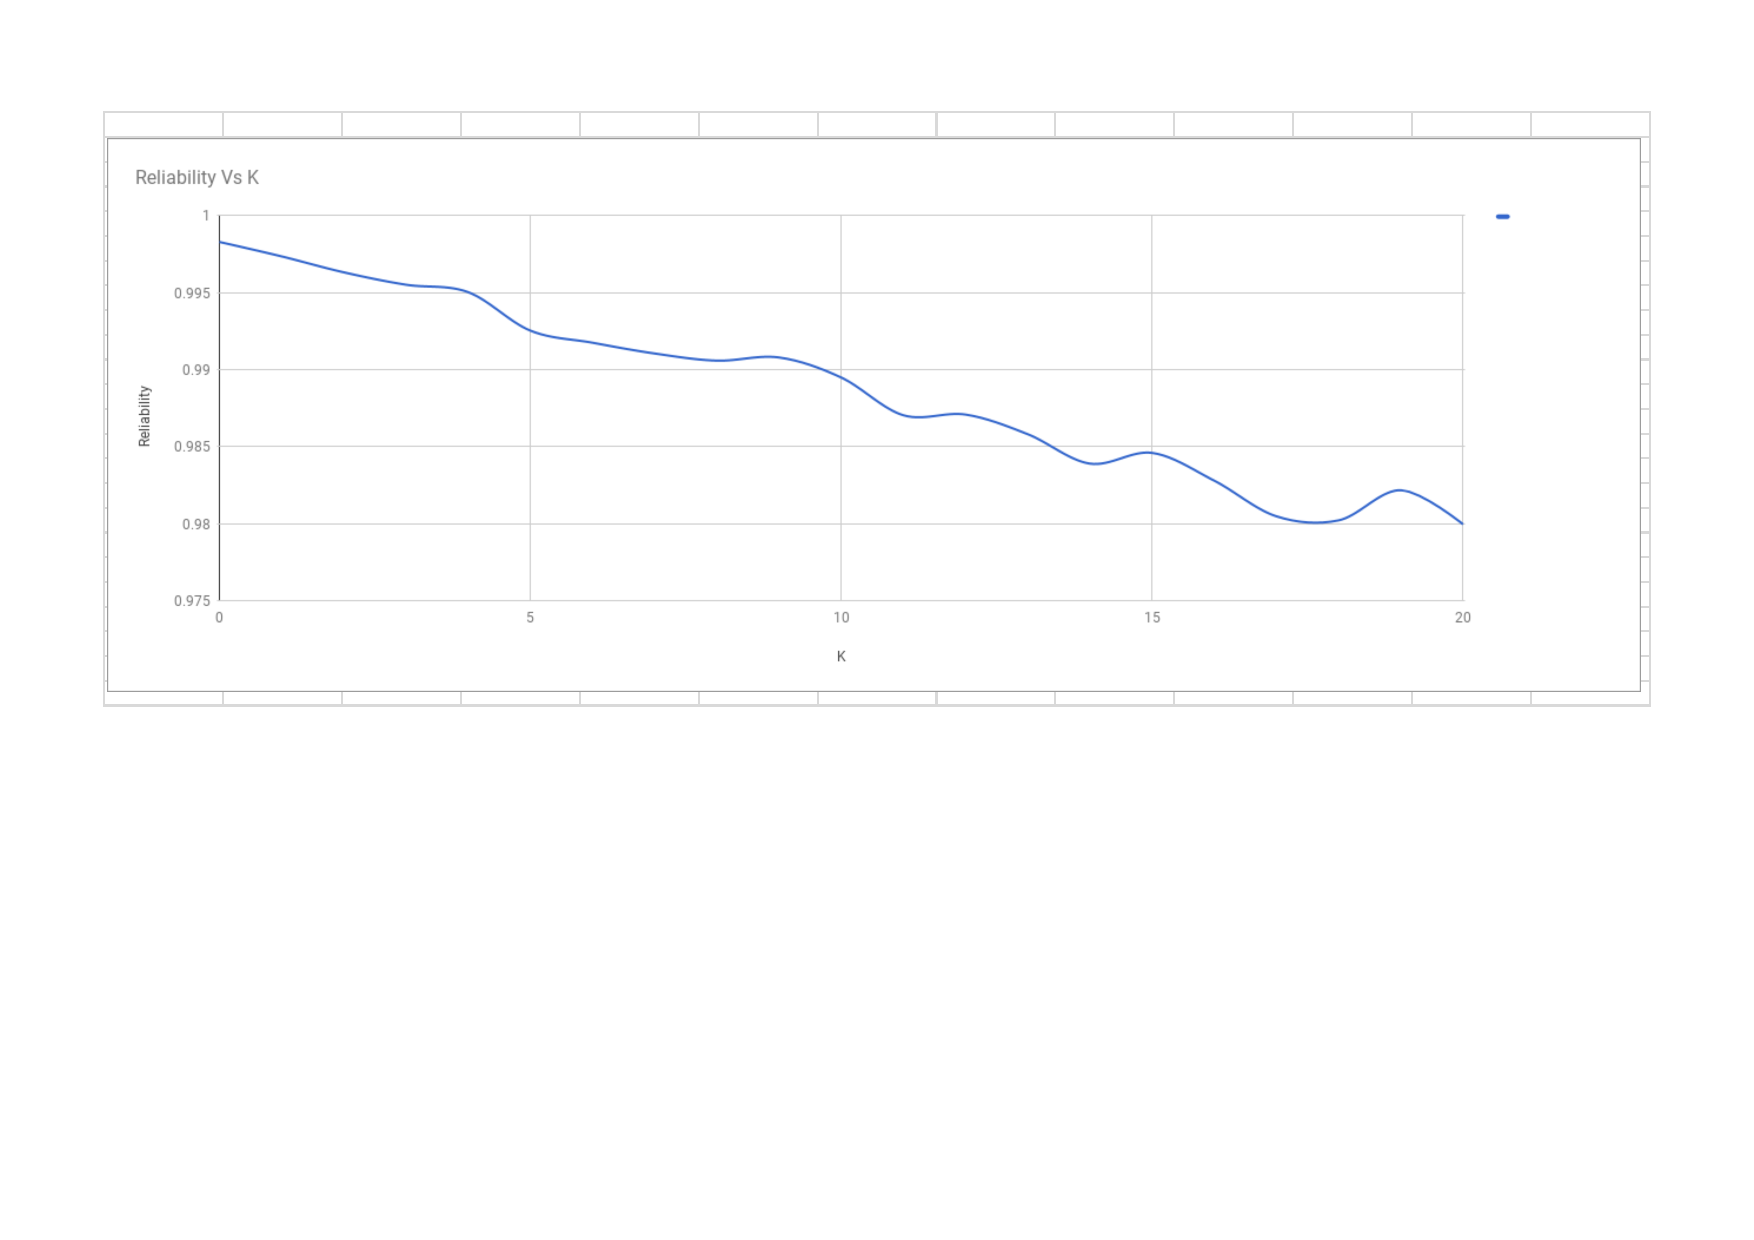
\includegraphics[width=\linewidth]{ReliabilityvsProbability.pdf}
\label{fig: kvr}
\caption{K vs Reliability}
\end{figure}
\begin{figure}
  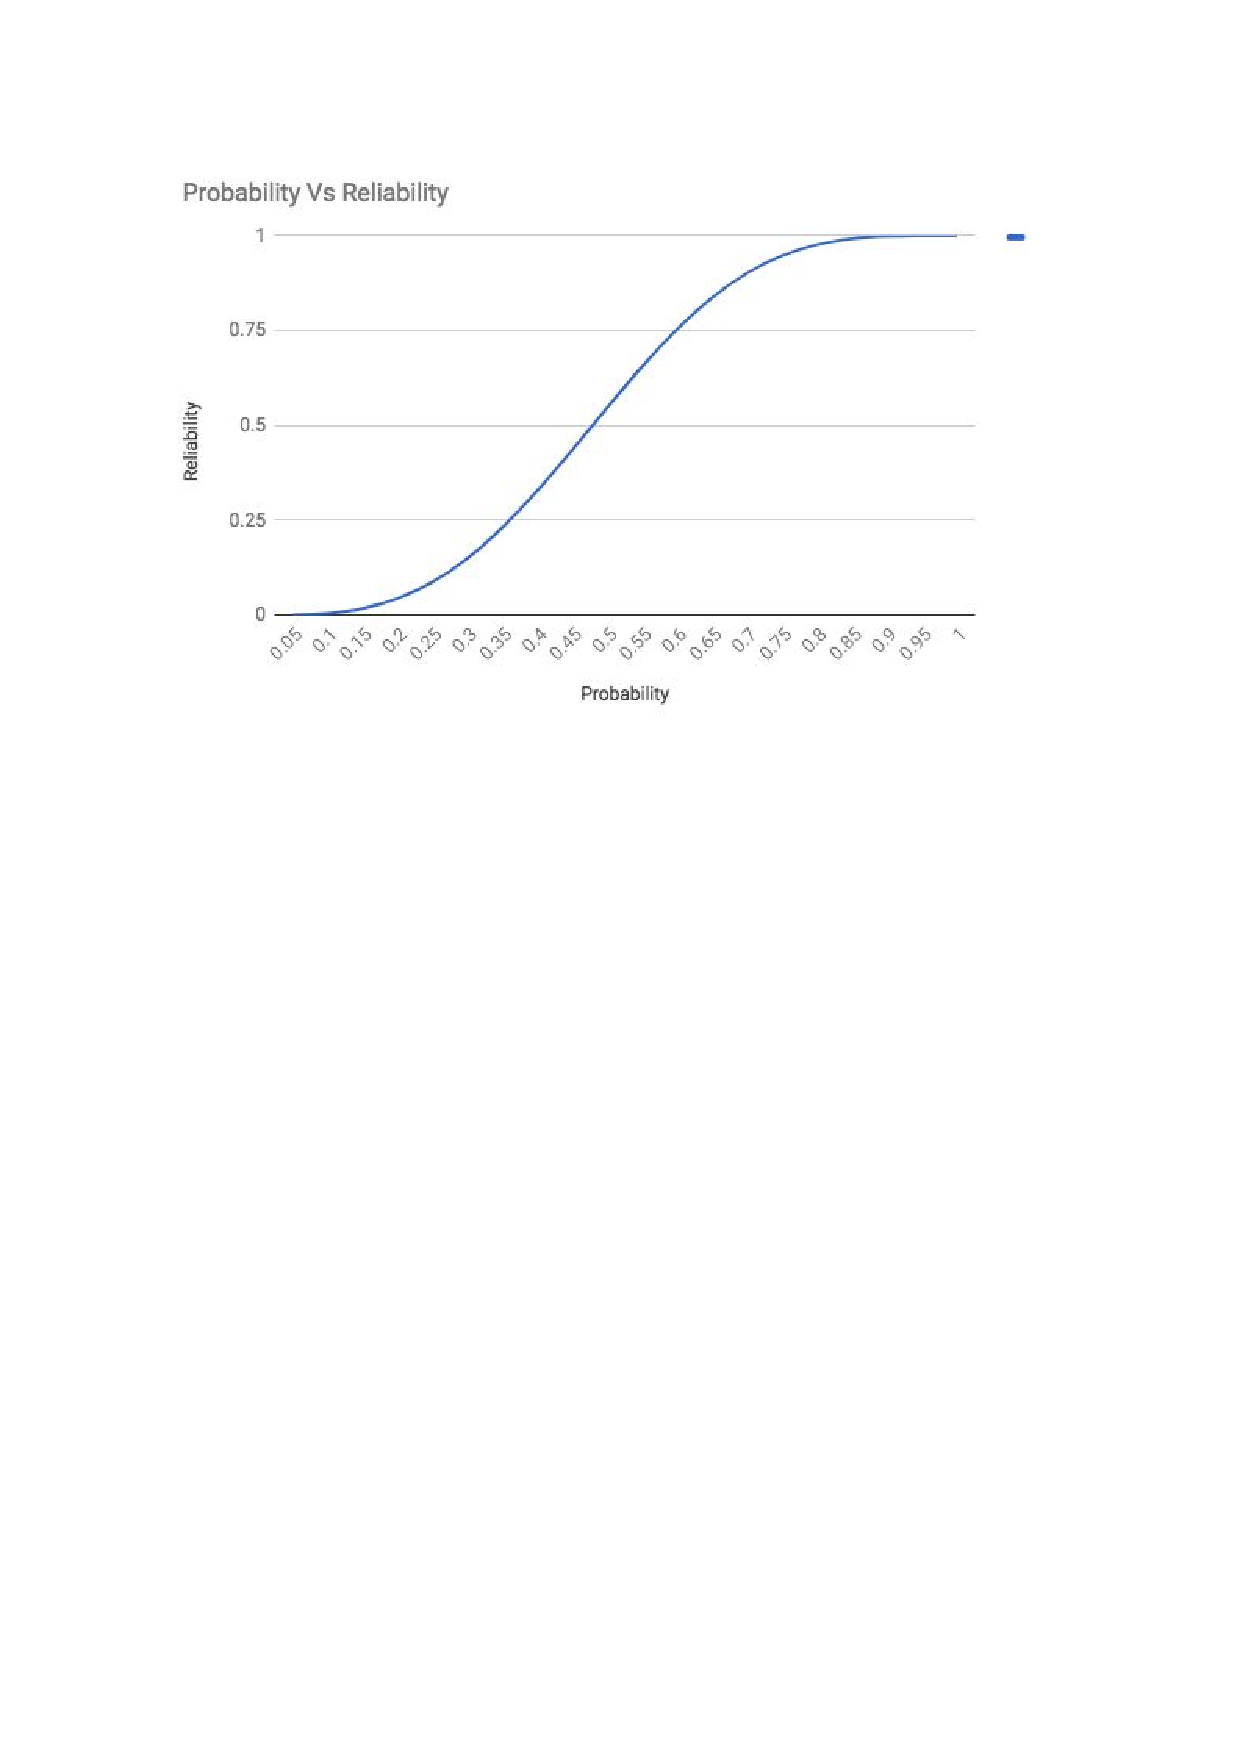
\includegraphics[width=\linewidth]{kvsreliability.pdf}
\label{fig: rvp}
\caption{Probability vs Reliability}
\end{figure}
\end{document}
 